\documentclass[10pt,twocolumn,a4paper]{article}

% ==============================================================================
% PACKAGES & CONFIGURATION
% ==============================================================================
\usepackage[utf8]{inputenc}
\usepackage[margin=1.8cm,top=2.2cm,bottom=2.2cm]{geometry}
\usepackage{amsmath,amssymb,amsfonts}
\usepackage{booktabs}
\usepackage{tabularx}
\usepackage{multirow}
\usepackage{microtype}
\usepackage{xcolor}
\usepackage{float}
\usepackage{caption}
\usepackage[hyphens]{url}
\usepackage{tikz}
\usetikzlibrary{arrows.meta,positioning,shapes.geometric,fit,backgrounds}
\usepackage{hyperref}
\usepackage{tcolorbox}
\usepackage{enumitem}
\usepackage{titlesec}
\usepackage{fancyhdr}

% Color Definitions for Minimal Industrial Palette
\definecolor{inkblack}{HTML}{111111}
\definecolor{deepslate}{HTML}{2D3748}
\definecolor{mutedtaupe}{HTML}{718096}
\definecolor{bordergray}{HTML}{E2E8F0}
\definecolor{surfacebg}{HTML}{F8FAFC}
\definecolor{criticalcoral}{HTML}{E53E3E}
\definecolor{warningamber}{HTML}{D69E2E}
\definecolor{successgreen}{HTML}{38A169}
\definecolor{accentblue}{HTML}{3182CE}

\hypersetup{
    colorlinks=true,
    linkcolor=deepslate,
    citecolor=accentblue,
    urlcolor=accentblue
}

% Typography & Header Formatting
\setlist{nosep,leftmargin=*}
\titleformat{\section}{\large\bfseries\color{inkblack}}{\thesection}{0.8em}{}[\titlerule]
\titleformat{\subsection}{\normalsize\bfseries\color{deepslate}}{\thesubsection}{0.6em}{}
\titleformat{\subsubsection}{\small\bfseries\color{deepslate}}{\thesubsubsection}{0.4em}{}

\pagestyle{fancy}
\fancyhf{}
\renewcommand{\headrulewidth}{0.4pt}
\renewcommand{\footrulewidth}{0.4pt}
\fancyhead[L]{\footnotesize\color{mutedtaupe}ManufactureFlow: Autonomous Manufacturing Resilience Control Plane}
\fancyhead[R]{\footnotesize\color{mutedtaupe}Technical Architecture \& Systems Study}
\fancyfoot[L]{\footnotesize\color{mutedtaupe}Version 1.0 (Audit Baseline)}
\fancyfoot[R]{\footnotesize\thepage}

% Classification Tag Command
\newcommand{\claimtag}[1]{%
    \textsf{\textbf{\scriptsize\color{deepslate}[#1]}}%
}

% ==============================================================================
% DOCUMENT BEGIN
% ==============================================================================
\begin{document}

% ------------------------------------------------------------------------------
% TITLE & METADATA BLOCK
% ------------------------------------------------------------------------------
\twocolumn[{%
\begin{center}
  {\LARGE\bfseries\color{inkblack} ManufactureFlow: An Autonomous Manufacturing Resilience Control Plane}\par\vspace{0.4em}
  {\large\color{deepslate} Event-Driven Failure Recovery Across Maintenance, Production, Procurement, and Customer Delivery}\par\vspace{0.8em}
  \rule{0.6\textwidth}{0.5pt}\par\vspace{0.8em}
  {\small\textbf{Engineering Architecture \& Applied Industrial Systems Study}}\par\vspace{0.2em}
  {\footnotesize Product: \textbf{ManufactureFlow / Machine Overwatch} \quad$|$\quad Domain: \textbf{Industrial Automation \& Autonomous Operations}}\par\vspace{0.2em}
  {\footnotesize Status: \textbf{Implementation Audit Baseline} \quad$|$\quad Classification: \textbf{Open Architecture Technical Report}}\par\vspace{1.2em}
\end{center}

\begin{quote}
  \small
  \textbf{Abstract}---In modern discrete manufacturing facilities, unexpected machine breakdown initiates an immediate cross-departmental cascade of operational disruptions, spanning line stoppages, spare shortages, procurement latency, scheduling bottlenecks, and missed customer shipments. Conventional industrial architectures isolate predictive maintenance (PdM) within diagnostic silos, leaving recovery orchestration to manual human intervention across fragmented Computerized Maintenance Management Systems (CMMS), Manufacturing Execution Systems (MES), and Enterprise Resource Planning (ERP) databases. This paper presents the architecture and implementation of \textbf{ManufactureFlow} (internally designated \textit{Machine Overwatch}), an autonomous manufacturing resilience control plane. By coupling continuous machine health telemetry monitoring with a deterministic, governed diagnostic provider and an idempotent multi-agent runtime compiled under LangGraph and persisted in PostgreSQL, the system reduces software-mediated coordination latency. When mechanical degradation is observed, the platform autonomously evaluates failure risk, issues allocation locks on compromised workstations, verifies warehouse inventory, triggers automated vendor procurement for stockout components, drafts critical work orders, dynamically calculates restoration timestamps, reroutes queued production jobs across qualified machines, and re-projects customer delivery commitments. Physical machine recovery is governed under strict human-in-the-loop Return-to-Service (RTS) validation. The state-graph architecture establishes an auditable, deterministic, and transactionally governed industrial control loop.
  \par\vspace{0.5em}
  \noindent\textbf{Keywords:} Predictive Maintenance, Manufacturing Resilience, Multi-Agent Systems, LangGraph, Production Rerouting, Dynamic Scheduling, Inventory Reservation, Industrial IoT, Human-in-the-Loop, Digital Twin, Transactional Control Plane.
\end{quote}
\vspace{1.2em}
}]

% ------------------------------------------------------------------------------
% 1. INTRODUCTION
% ------------------------------------------------------------------------------
\section{Introduction}
\label{sec:introduction}
Discrete manufacturing operations rely on synchronized workstation networks where work-in-progress (WIP) progresses sequentially through machining, surface treatment, assembly, and inspection cells. Under this physical coupling, the sudden failure of an individual workstation is never an isolated mechanical event. Rather, equipment downtime propagates instantly across operational boundaries, impacting factory throughput, component availability, labor allocations, and downstream shipment windows.

Historically, industrial automation has focused on isolated instrumentation: Supervisory Control and Data Acquisition (SCADA) platforms collect telemetry, while condition-monitoring tools detect anomalous vibration or thermal signatures. However, these systems are fundamentally passive; they emit visual alarms on monitoring dashboards but lack the cross-domain authority to intercept the operational cascade. Consequently, the burden of failure response falls upon human operators. Shift supervisors must investigate root causes, maintenance planners inspect warehouse bins, procurement buyers negotiate emergency purchase orders, production schedulers manually adjust spreadsheets, and logistics officers discover delivery delays after deadlines have already lapsed. This operational coordination latency routinely exceeds the physical wrench-time required for machine repair by an order of magnitude.

ManufactureFlow addresses this structural gap by functioning as an \textit{Autonomous Manufacturing Resilience Control Plane}. Rather than treating predictive maintenance as an alert generator, the platform establishes an event-driven, closed-loop state machine. Software agents autonomously execute multi-departmental recovery logic within strict deterministic constraints, while human specialists retain final authority over physical repairs and return-to-service validation.

The primary contribution of this work is:
\begin{quote}
\textit{A deterministic, transactionally governed agentic control plane that converts machine-health events into cross-domain recovery actions within sub-second digital orchestration latency while preserving human authority over physical restoration.}
\end{quote}

% ------------------------------------------------------------------------------
% 2. SYSTEM SCOPE & CLAIM CLASSIFICATION
% ------------------------------------------------------------------------------
\section{System Scope \& Claim Classification}
\label{sec:scope}
To maintain rigorous engineering truth and auditability, this technical report enforces a strict taxonomy of technical claims across all sections:

\begin{itemize}
    \item \claimtag{IMPLEMENTED}: Fully executable backend logic integrated into the codebase, maintaining state persistence in PostgreSQL.
    \item \claimtag{CONTROLLED}: Standardized operational scenario execution using governed diagnostic fixtures (e.g., standard industrial test fixture WS-102).
    \item \claimtag{MEASURED}: Quantitatively measured runtime latency and execution integrity benchmarked on the test harness.
    \item \claimtag{VERIFIED}: Formally verified across automated test suites for invariant consistency and idempotency.
    \item \claimtag{TARGET}: Enterprise operational benchmark criteria defined in the industrial requirements specification (\texttt{docs/PS.md}).
\end{itemize}

Crucially, this report distinguishes between \textbf{digital orchestration latency} (the programmatic execution of state transitions, constraint evaluations, and database writes) and \textbf{physical recovery latency} (the mechanical wrench-time, technician dispatch, part transit, and testing required to physically restore equipment).

% ------------------------------------------------------------------------------
% 3. PROBLEM FORMULATION & FAILURE CASCADE
% ------------------------------------------------------------------------------
\section{Problem Formulation}
\label{sec:problem_formulation}
To model the systemic vulnerability of conventional manufacturing operations, we formalize the operational failure cascade as a coupled temporal-state dependency chain.

\subsection{Formal Failure Cascade Model}
Let a manufacturing plant be modeled as a tuple $\mathcal{P} = (\mathcal{W}, \mathcal{J}, \mathcal{I}, \mathcal{V}, \mathcal{S})$, representing workstations, production jobs, inventory stocks, approved vendors, and customer shipment commitments. 

\begin{enumerate}
    \item \textbf{Degradation Inception}: A mechanical component on workstation $w_i \in \mathcal{W}$ experiences physical wear, manifested as anomalous telemetry $\mathbf{x}(t) = [T, V, I, P]^\top$ exceeding safe operational bounds $\mathbf{\theta}_{\text{safe}}$.
    \item \textbf{Availability Disruption}: The equipment transitions to an unviable state, causing immediate unavailability $\alpha(w_i) \to 0$.
    \item \textbf{Work-in-Progress Freeze}: All assigned active and queued jobs $\mathcal{J}(w_i) \subset \mathcal{J}$ are suspended, halting downstream line feed.
    \item \textbf{Spare Inventory Contention}: Remediation requires specific component $p_k$. The inventory state $q(p_k)$ must satisfy $q(p_k) \ge r_{\text{req}}$. If $q(p_k) = 0$, an emergency procurement cycle is initiated with lead time $\tau_{\text{lead}}(v_m)$, where $v_m \in \mathcal{V}$.
    \item \textbf{Restoration Latency}: Total workstation downtime $\tau_{\text{down}}$ becomes a function of procurement latency, physical repair duration $\tau_{\text{repair}}$, and testing duration $\tau_{\text{test}}$:
    \begin{equation}
        \tau_{\text{down}} = \mathbb{I}_{\{q(p_k) = 0\}} \cdot \tau_{\text{lead}}(v_m) + \tau_{\text{inspect}} + \tau_{\text{repair}} + \tau_{\text{test}}
    \end{equation}
    \item \textbf{Delivery Compromise}: Shipment $s_l \in \mathcal{S}$ depends on completion times of jobs $J_s \subset \mathcal{J}$. The delay propagates to customer delivery commitments:
    \begin{equation}
        t_{\text{proj}}(s_l) = \max_{j \in J_s} \{ t_{\text{comp}}(j) \} + \tau_{\text{post}}
    \end{equation}
    When $t_{\text{proj}}(s_l) > t_{\text{commit}}(s_l)$, a delivery breach occurs.
\end{enumerate}

\begin{figure}[H]
\centering
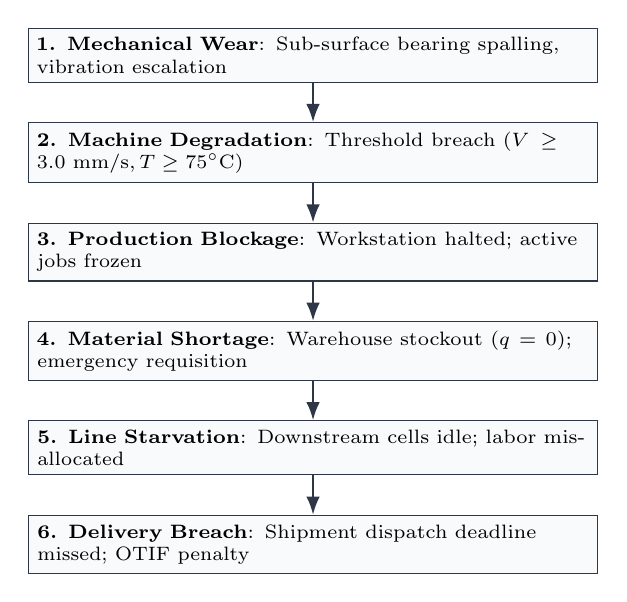
\begin{tikzpicture}[
    node distance=0.5cm,
    block/.style={rectangle, draw=deepslate, fill=surfacebg, text width=7cm, font=\scriptsize, minimum height=0.45cm, align=left},
    arrow/.style={-Latex, deepslate, thick}
]
\node[block] (n1) {\textbf{1. Mechanical Wear}: Sub-surface bearing spalling, vibration escalation};
\node[block, below=of n1] (n2) {\textbf{2. Machine Degradation}: Threshold breach ($V \ge 3.0\text{ mm/s}, T \ge 75^\circ\text{C}$)};
\node[block, below=of n2] (n3) {\textbf{3. Production Blockage}: Workstation halted; active jobs frozen};
\node[block, below=of n3] (n4) {\textbf{4. Material Shortage}: Warehouse stockout ($q=0$); emergency requisition};
\node[block, below=of n4] (n5) {\textbf{5. Line Starvation}: Downstream cells idle; labor misallocated};
\node[block, below=of n5] (n6) {\textbf{6. Delivery Breach}: Shipment dispatch deadline missed; OTIF penalty};

\draw[arrow] (n1) -- (n2);
\draw[arrow] (n2) -- (n3);
\draw[arrow] (n3) -- (n4);
\draw[arrow] (n4) -- (n5);
\draw[arrow] (n5) -- (n6);
\end{tikzpicture}
\caption{The Industrial Failure Cascade: Unmitigated degradation propagating across operational, supply-chain, and customer delivery domains.\label{fig:failure_cascade}}
\end{figure}

The foundational research question investigated in this study is:
\begin{quote}
\textit{Can an autonomous, event-driven state graph digitally initiate and coordinate the recovery cascade within sub-second orchestration latency while preserving deterministic operational safety constraints?}
\end{quote}

% ------------------------------------------------------------------------------
% 4. SYSTEM OBJECTIVES
% ------------------------------------------------------------------------------
\section{System Objectives}
\label{sec:objectives}
Table~\ref{tab:system_objectives} delineates the operational objectives of ManufactureFlow, mapping business requirements to concrete system mechanisms and implementation evidence.

\begin{table*}[t]
\centering
\scriptsize
\caption{System Objectives and Engineering Execution Matrix\label{tab:system_objectives}}
\begin{tabularx}{\textwidth}{lXXl}
\toprule
\textbf{Objective} & \textbf{Operational Requirement} & \textbf{System Mechanism} & \textbf{Implementation Status} \\
\midrule
Early Anomaly Detection & Identify pre-breakdown degradation & Telemetry ingestion \& multi-sensor threshold evaluation & \claimtag{IMPLEMENTED} \\
Fault Diagnostics & Identify failing component and TTF & Diagnostic provider abstraction with risk scoring & \claimtag{CONTROLLED} \\
Asset Protection & Prevent loading jobs on degraded machines & ACID-compliant allocation lock on workstation entity & \claimtag{IMPLEMENTED} \\
Spare Availability & Commit parts before technician dispatch & Optimistic locking \& reservation on warehouse items & \claimtag{IMPLEMENTED} \\
Procurement Automation & Automate vendor POs upon stockout & Deterministic vendor ranking (lead, cost, reliability) & \claimtag{IMPLEMENTED} \\
Maintenance Planning & Provide structured checklists & Critical work-order creation with LOTO checklists & \claimtag{IMPLEMENTED} \\
Restoration Estimation & Dynamic recovery date calculation & Versioned mathematical model with SHA-256 input hashing & \claimtag{IMPLEMENTED} \\
Production Continuity & Reroute work to qualified cells & Multi-constraint candidate ranking (tools, skills, load) & \claimtag{IMPLEMENTED} \\
Logistics Visibility & Determine customer shipment delay & Temporal propagation engine classifying delivery margin & \claimtag{IMPLEMENTED} \\
Stakeholder Alignment & Push actionable notifications & Role-based notification queue (Scheduler, Logistics, Lead) & \claimtag{IMPLEMENTED} \\
Audit Governance & Provide full incident lineage & Monotonic event-store keyed by unique correlation ID & \claimtag{IMPLEMENTED} \\
\bottomrule
\end{tabularx}
\end{table*}

% ------------------------------------------------------------------------------
% 5. SYSTEM ARCHITECTURE
% ------------------------------------------------------------------------------
\section{System Architecture}
\label{sec:architecture}
ManufactureFlow is implemented as a multi-tier, modular enterprise-style architecture decoupling user visualization, state-graph orchestration, domain business logic, and transactional persistence.

\begin{figure*}[t]
\centering
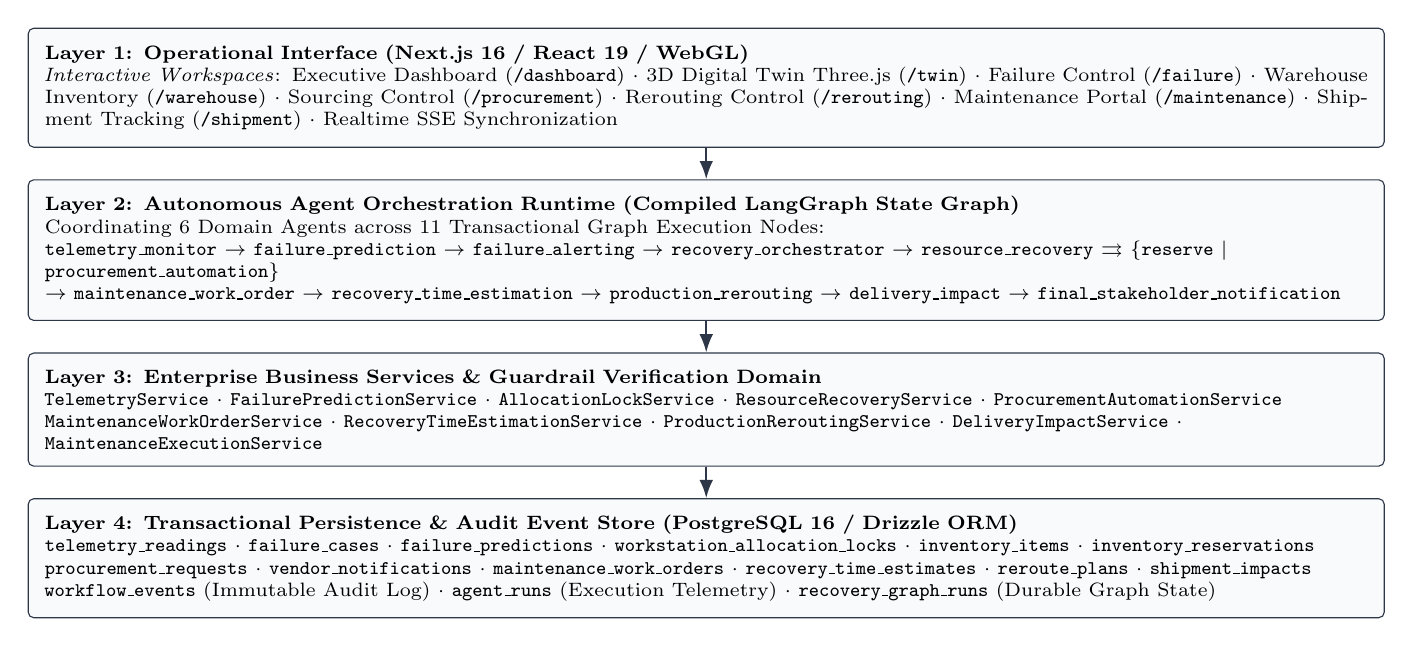
\begin{tikzpicture}[
    node distance=0.4cm,
    layer/.style={rectangle, draw=deepslate, fill=surfacebg, rounded corners=2pt, inner sep=6pt, font=\scriptsize},
    title/.style={font=\bfseries\scriptsize\color{inkblack}}
]

% Layer 1: Interface
\node[layer, text width=16.8cm] (ui) {
    \textbf{Layer 1: Operational Interface (Next.js 16 / React 19 / WebGL)}\\
    \textit{Interactive Workspaces}: Executive Dashboard (\texttt{/dashboard}) $\cdot$ 3D Digital Twin Three.js (\texttt{/twin}) $\cdot$ Failure Control (\texttt{/failure}) $\cdot$ Warehouse Inventory (\texttt{/warehouse}) $\cdot$ Sourcing Control (\texttt{/procurement}) $\cdot$ Rerouting Control (\texttt{/rerouting}) $\cdot$ Maintenance Portal (\texttt{/maintenance}) $\cdot$ Shipment Tracking (\texttt{/shipment}) $\cdot$ Realtime SSE Synchronization
};

% Layer 2: Orchestration
\node[layer, text width=16.8cm, below=of ui] (orch) {
    \textbf{Layer 2: Autonomous Agent Orchestration Runtime (Compiled LangGraph State Graph)}\\
    Coordinating 6 Domain Agents across 11 Transactional Graph Execution Nodes:\\
    \texttt{telemetry\_monitor} $\to$ \texttt{failure\_prediction} $\to$ \texttt{failure\_alerting} $\to$ \texttt{recovery\_orchestrator} $\to$ \texttt{resource\_recovery} $\rightrightarrows$ \{\texttt{reserve} $|$ \texttt{procurement\_automation}\}\\
    $\to$ \texttt{maintenance\_work\_order} $\to$ \texttt{recovery\_time\_estimation} $\to$ \texttt{production\_rerouting} $\to$ \texttt{delivery\_impact} $\to$ \texttt{final\_stakeholder\_notification}
};

% Layer 3: Services
\node[layer, text width=16.8cm, below=of orch] (services) {
    \textbf{Layer 3: Enterprise Business Services \& Guardrail Verification Domain}\\
    \texttt{TelemetryService} $\cdot$ \texttt{FailurePredictionService} $\cdot$ \texttt{AllocationLockService} $\cdot$ \texttt{ResourceRecoveryService} $\cdot$ \texttt{ProcurementAutomationService}\\
    \texttt{MaintenanceWorkOrderService} $\cdot$ \texttt{RecoveryTimeEstimationService} $\cdot$ \texttt{ProductionReroutingService} $\cdot$ \texttt{DeliveryImpactService} $\cdot$ \texttt{MaintenanceExecutionService}
};

% Layer 4: Persistence
\node[layer, text width=16.8cm, below=of services] (data) {
    \textbf{Layer 4: Transactional Persistence \& Audit Event Store (PostgreSQL 16 / Drizzle ORM)}\\
    \texttt{telemetry\_readings} $\cdot$ \texttt{failure\_cases} $\cdot$ \texttt{failure\_predictions} $\cdot$ \texttt{workstation\_allocation\_locks} $\cdot$ \texttt{inventory\_items} $\cdot$ \texttt{inventory\_reservations} \\
    \texttt{procurement\_requests} $\cdot$ \texttt{vendor\_notifications} $\cdot$ \texttt{maintenance\_work\_orders} $\cdot$ \texttt{recovery\_time\_estimates} $\cdot$ \texttt{reroute\_plans} $\cdot$ \texttt{shipment\_impacts} \\
    \texttt{workflow\_events} (Immutable Audit Log) $\cdot$ \texttt{agent\_runs} (Execution Telemetry) $\cdot$ \texttt{recovery\_graph\_runs} (Durable Graph State)
};

\draw[-Latex, thick, deepslate] (ui) -- (orch);
\draw[-Latex, thick, deepslate] (orch) -- (services);
\draw[-Latex, thick, deepslate] (services) -- (data);

\end{tikzpicture}
\caption{Four-Tier Enterprise Architecture of ManufactureFlow, illustrating separation of presentation, state-graph orchestration, business services, and ACID persistence.\label{fig:system_architecture}}
\end{figure*}

\subsection{Architectural Decoupling Principles}
\begin{itemize}
    \item \textbf{Stateless Execution with External Persistence}: The application workers are stateless between invocations; workflow state is externally persisted and reconstructed from PostgreSQL checkpointers and durable execution records (\texttt{recovery\_graph\_runs}, \texttt{agent\_runs}). Every graph node receives a strictly typed context (\texttt{RecoveryGraphState}), executes domain logic via Layer~3 services, writes state changes to PostgreSQL, and returns state patches.
    \item \textbf{Dual-Database Logical Isolation}: The system maintains two logically isolated PostgreSQL databases, \texttt{machine\_overwatch} (Live) and \texttt{machine\_overwatch\_demo} (Demo), hosted on the same PostgreSQL server instance accessed through port 5434. Application runtime configuration (\texttt{APP\_RUNTIME=live} vs. \texttt{APP\_RUNTIME=demo}) selects the active database at startup. This guarantees that simulation ticks and interactive demonstration runs never mutate or pollute live operational baselines.
    \item \textbf{Server-Sent Events (SSE) Bus}: Connects client browser contexts to the backend event stream (\texttt{/api/events}), broadcasting state mutations in real time without polling overhead.
\end{itemize}

% ------------------------------------------------------------------------------
% 6. CORE AGENT SUITE & ORCHESTRATION RUNTIME
% ------------------------------------------------------------------------------
\section{Autonomous Agent Suite \& Runtime}
\label{sec:agents}
A critical architectural distinction in ManufactureFlow is the decoupling between \textbf{autonomous domain agents}, \textbf{transactional graph execution nodes}, and \textbf{deterministic domain services/tools}. The platform architecture comprises \textbf{six specialized agents} operating under clear functional boundaries:

\begin{enumerate}
    \item \textbf{Failure Intelligence Agent}: Ingests incoming sensor telemetry, verifies schema validity, evaluates physical parameter thresholds, queries the diagnostic provider boundary for failure modes, and estimates the Time-to-Failure (TTF). It encapsulates graph nodes \texttt{telemetry\_monitor}, \texttt{failure\_prediction}, and \texttt{failure\_alerting}.
    \item \textbf{Recovery Orchestrator Agent}: Evaluates diagnostic severity against operational safety guardrails ($P \ge 85\%$, $\text{TTF} \le 24\text{h}$); acquires transactional allocation locks on compromised workstations to prevent job releases.
    \item \textbf{Resource Recovery Agent}: Coordinates spare part resolution and physical remediation planning. Rather than fragmenting into separate agents, this agent orchestrates four deterministic domain services:
    \begin{itemize}
        \item \textit{Inventory Reservation Service}: Queries warehouse stock and acquires optimistic row locks.
        \item \textit{Procurement Automation Service}: Evaluates approved suppliers using an objective ranking function of lead time, cost, and reliability score; drafts purchase requisitions upon stockout.
        \item \textit{Maintenance Work Order Service}: Synthesizes critical work orders incorporating lockout-tagout (LOTO) checklists aligned with OSHA 29 CFR 1910.147 principles.
        \item \textit{Recovery Time Estimation Service}: Computes deterministic expected recovery timestamps via versioned mathematical models stamped with a SHA-256 parameter hash.
    \end{itemize}
    \item \textbf{Production Rerouting Agent}: Evaluates alternative workstations for operational qualification (tooling, operator skill certifications) and available capacity; executes atomic job reassignment.
    \item \textbf{Delivery Impact Agent}: Traverses downstream order dependencies, projects completion time deviations against customer delivery SLAs, and classifies delivery risks.
    \item \textbf{Stakeholder Notification Agent}: Formats and persists structured, role-specific operational alerts targeted to Plant Managers, Maintenance Leads, Schedulers, and Logistics Officers.
\end{enumerate}

The orchestration runtime decomposes the recovery workflow into \textbf{11 discrete transactional execution nodes} within a compiled LangGraph state machine (\path{backend/src/lib/agent-graph/graph.ts}). Several graph nodes invoke deterministic services owned by the Resource Recovery Agent rather than representing independent autonomous agents. This architectural discipline prevents logic sprawl and ensures that deterministic mathematical tasks remain isolated in testable domain services.

\begin{table*}[t]
\centering
\scriptsize
\caption{Agent Responsibility, Operational Boundary, and Guardrail Matrix\label{tab:agent_matrix}}
\begin{tabularx}{\textwidth}{>{\raggedright\arraybackslash}p{2.4cm}XXXX>{\raggedright\arraybackslash}X>{\raggedright\arraybackslash}p{1.8cm}}
\toprule
\textbf{Agent / Tool} & \textbf{Trigger} & \textbf{Inputs Consumed} & \textbf{Operational Decision} & \textbf{Automated Action} & \textbf{Enforced Guardrails} & \textbf{Status} \\
\midrule
Failure Intelligence Agent & Telemetry Ingestion & $\mathbf{x}=[T, V, I, P]^\top$, Error Codes & Signal anomaly severity, failing part, TTF & Writes \texttt{failure\_cases} \& drafts alerts & Fixed physical threshold bounds & \claimtag{CONTROLLED} \\
Recovery Orchestrator Agent & Validated Prediction & Severity, Probability, TTF & Determine if machine must be locked & Writes \texttt{allocation\_lock}; status $\to$ \texttt{SHUTDOWN} & $P \ge 85\% \land \text{TTF} \le 24\text{h}$ & \claimtag{IMPLEMENTED} \\
Resource Recovery Agent & Allocation Lock & Part code, plant ID, quantity & Select local spare or procurement branch & Coordinates inventory, procurement, WO, ETA & Optimistic DB row lock ($q \ge r$) & \claimtag{IMPLEMENTED} \\
\quad \textit{-- Inventory Tool} & Inventory Check & Part number, required quantity & Reserve local stock if available & Increments reserved stock in DB & On-hand minus reserved $\ge$ required & \claimtag{IMPLEMENTED} \\
\quad \textit{-- Procurement Tool} & Stockout ($q=0$) & Part number, approved vendors & Rank vendors (lead, cost, reliability) & Drafts purchase requisition & Active, approved vendor capabilities & \claimtag{IMPLEMENTED} \\
\quad \textit{-- Work Order Tool} & Part Reserved/Ordered & Part, fault, machine, priority & Generate maintenance tasks \& LOTO & Creates work order in stage \texttt{PLANNED} & Valid time window, safety checklist & \claimtag{IMPLEMENTED} \\
\quad \textit{-- Recovery ETA Tool} & Work Order Created & Lead time, repair, test durations & Calculate expected recovery timestamp & Writes estimate with SHA-256 hash & Monotonic duration, window constraints & \claimtag{IMPLEMENTED} \\
Production Rerouting Agent & Recovery Estimate & Source station, affected jobs & Candidate matching \& load balancing & Reassigns jobs, updates station loads & Strict tooling, skill, capacity $\le 100\%$ & \claimtag{IMPLEMENTED} \\
Delivery Impact Agent & Reroute Executed & Job completion projections, commitments & Shipment risk (\texttt{ON\_TIME}, \texttt{DELAYED}) & Writes \texttt{shipment\_impacts} \& notifies & Mathematical delta against order SLA & \claimtag{IMPLEMENTED} \\
Stakeholder Notification Agent & Recovery Complete & Multi-department recovery state & Target role alerts (Scheduler, Plant, etc.) & Inserts records into \texttt{notifications} & Role-specific payload schema & \claimtag{IMPLEMENTED} \\
\bottomrule
\end{tabularx}
\end{table*}

% ------------------------------------------------------------------------------
% 7. END-TO-END WORKFLOW & STATE TRANSITION
% ------------------------------------------------------------------------------
\section{End-to-End Recovery Workflow}
\label{sec:workflow}
The recovery lifecycle executes as an idempotent state transition. Figure~\ref{fig:workflow_state_graph} illustrates the compiled LangGraph routing topology, highlighting the conceptual 6-agent hierarchy and distinguishing automated logic, transactional writes, and human-gated checkpoints.

\begin{figure*}[t]
\centering
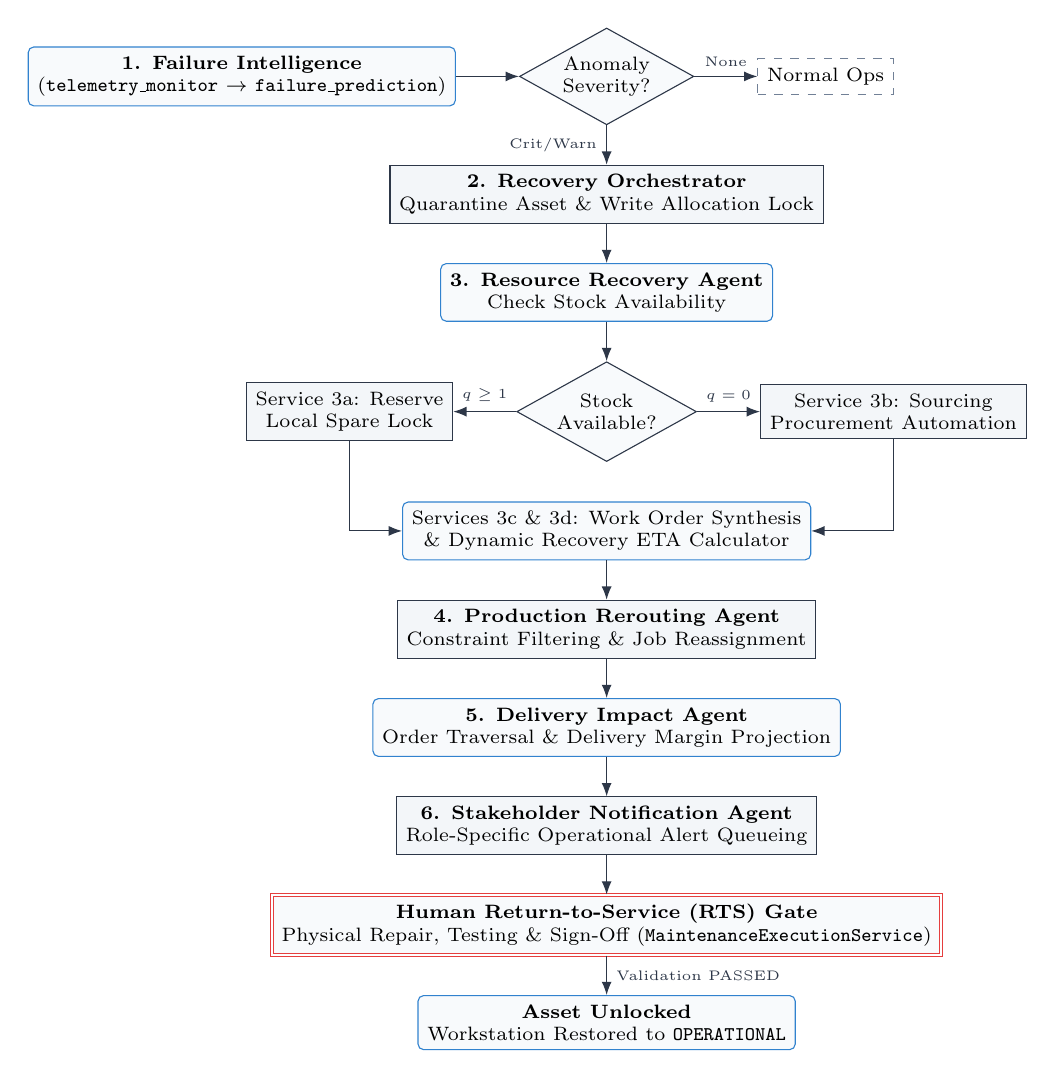
\begin{tikzpicture}[
    node distance=0.5cm and 0.8cm,
    agent_box/.style={rectangle, draw=accentblue, fill=surfacebg, rounded corners=2pt, font=\scriptsize, align=center, minimum height=0.6cm},
    tx_box/.style={rectangle, draw=deepslate, fill=bordergray!40, font=\scriptsize, align=center, minimum height=0.6cm},
    human_box/.style={rectangle, draw=criticalcoral, fill=surfacebg, double, font=\scriptsize, align=center, minimum height=0.6cm},
    decision/.style={diamond, draw=deepslate, fill=surfacebg, aspect=1.8, inner sep=1pt, font=\scriptsize, align=center},
    arrow/.style={-Latex, deepslate, font=\tiny}
]

% Agent 1
\node[agent_box] (ag1) {\textbf{1. Failure Intelligence}\\(\texttt{telemetry\_monitor} $\to$ \texttt{failure\_prediction})};
\node[decision, right=of ag1] (anom_check) {Anomaly\\Severity?};
\node[rectangle, draw=mutedtaupe, dashed, right=of anom_check, font=\scriptsize] (term_normal) {Normal Ops};

% Agent 2
\node[tx_box, below=of anom_check] (ag2) {\textbf{2. Recovery Orchestrator}\\Quarantine Asset \& Write Allocation Lock};

% Agent 3
\node[agent_box, below=of ag2] (ag3) {\textbf{3. Resource Recovery Agent}\\Check Stock Availability};
\node[decision, below=of ag3] (stock_check) {Stock\\Available?};

\node[tx_box, left=of stock_check] (reserve) {Service 3a: Reserve\\Local Spare Lock};
\node[tx_box, right=of stock_check] (procure) {Service 3b: Sourcing\\Procurement Automation};

\node[agent_box, below=of stock_check] (ag3_cont) {Services 3c \& 3d: Work Order Synthesis\\\& Dynamic Recovery ETA Calculator};

% Agent 4
\node[tx_box, below=of ag3_cont] (ag4) {\textbf{4. Production Rerouting Agent}\\Constraint Filtering \& Job Reassignment};

% Agent 5
\node[agent_box, below=of ag4] (ag5) {\textbf{5. Delivery Impact Agent}\\Order Traversal \& Delivery Margin Projection};

% Agent 6
\node[tx_box, below=of ag5] (ag6) {\textbf{6. Stakeholder Notification Agent}\\Role-Specific Operational Alert Queueing};

% Human RTS
\node[human_box, below=of ag6] (rts) {\textbf{Human Return-to-Service (RTS) Gate}\\Physical Repair, Testing \& Sign-Off (\texttt{MaintenanceExecutionService})};
\node[agent_box, below=of rts] (release) {\textbf{Asset Unlocked}\\Workstation Restored to \texttt{OPERATIONAL}};

% Connections
\draw[arrow] (ag1) -- (anom_check);
\draw[arrow] (anom_check) -- node[above]{None} (term_normal);
\draw[arrow] (anom_check) -- node[left]{Crit/Warn} (ag2);
\draw[arrow] (ag2) -- (ag3);
\draw[arrow] (ag3) -- (stock_check);
\draw[arrow] (stock_check) -- node[above]{$q \ge 1$} (reserve);
\draw[arrow] (stock_check) -- node[above]{$q = 0$} (procure);
\draw[arrow] (reserve) |- (ag3_cont);
\draw[arrow] (procure) |- (ag3_cont);
\draw[arrow] (ag3_cont) -- (ag4);
\draw[arrow] (ag4) -- (ag5);
\draw[arrow] (ag5) -- (ag6);
\draw[arrow] (ag6) -- (rts);
\draw[arrow] (rts) -- node[right]{Validation PASSED} (release);

\end{tikzpicture}
\caption{Compiled LangGraph Execution Flow. Blue outlines denote autonomous agent boundaries; shaded boxes denote transactional database updates; double red outlines denote human-in-the-loop authorization gates.\label{fig:workflow_state_graph}}
\end{figure*}

% ------------------------------------------------------------------------------
% 8. EXPERIMENTAL / CONTROLLED SCENARIO: WS-102
% ------------------------------------------------------------------------------
\section{Controlled Demonstration: Workstation WS-102}
\label{sec:scenario_ws102}
To validate the end-to-end operational flow, the platform implements a standardized industrial demonstration scenario centered on workstation \texttt{WS-102}.

\subsection{Baseline Asset Configuration}
\begin{itemize}
    \item \textbf{Machine Identity}: CNC Lathe Alpha (\texttt{WS-102}), Production Line L-03.
    \item \textbf{Initial Operational State}: Status \texttt{OPERATIONAL}, Capacity Utilization $62\%$.
    \item \textbf{Active Production Load}: Three production orders queued/in-flight:
    \begin{itemize}
        \item \texttt{J1001}: Operation \texttt{CNC-TURN}, Tooling \texttt{TL-XA}, Skill \texttt{CNC-L2}, Load $16\%$.
        \item \texttt{J1002}: Operation \texttt{CNC-TURN}, Tooling \texttt{TL-XA}, Skill \texttt{CNC-L2}, Load $14\%$.
        \item \texttt{J1003}: Operation \texttt{CNC-TURN}, Tooling \texttt{TL-XA}, Skill \texttt{CNC-L2}, Load $12\%$.
    \end{itemize}
\end{itemize}

\subsection{Observed Telemetry Injection}
The degradation vector injected into \texttt{/api/telemetry} reports physical parameter drift:
\begin{align*}
    T &= 79.0^\circ\text{C} \quad (\theta_{\text{crit}} = 75.0^\circ\text{C}) \\
    V &= 4.2\text{ mm/s} \quad (\theta_{\text{crit}} = 3.0\text{ mm/s}) \\
    I &= 22.0\text{ A} \quad (\theta_{\text{crit}} = 20.0\text{ A}) \\
    P &= 5.2\text{ bar} \quad (\text{Nominal: } [2.5, 8.5]) \\
    \text{Error} &= [\texttt{X\_AXIS\_VIBRATION}]
\end{align*}

\subsection{Controlled Diagnostic Resolution}
The telemetry triggers the diagnostic provider boundary (\texttt{ControlledFailurePredictionProvider}):
\begin{itemize}
    \item \textbf{Identified Root Cause}: Spindle Bearing Degradation
    \item \textbf{Required Part Number}: \texttt{BRG-10023}
    \item \textbf{Controlled Diagnostic Risk Score}: $0.92$ (Provider-returned controlled failure probability: $92\%$). \textit{This value is a deterministic scenario parameter and is not an empirically calibrated probability.}
    \item \textbf{Estimated Time-to-Failure (TTF)}: $\tau_{\text{ttf}} = 18.0\text{ Hours}$
    \item \textbf{Severity Level}: \texttt{CRITICAL}
\end{itemize}

% ------------------------------------------------------------------------------
% 9. DECISION LOGIC & SAFETY GUARDRAILS
% ------------------------------------------------------------------------------
\section{Decision Logic \& Safety Guardrails}
\label{sec:safety_model}
To prevent catastrophic asset damage and avoid false-positive shutdowns, the Recovery Orchestrator enforces a deterministic safety evaluation function $\Phi(s, p, \tau_{\text{ttf}})$:

\begin{equation}
\Phi = \begin{cases} 
\text{QUARANTINE} & \text{if } (s = \text{CRIT} \land p \ge 0.85 \\
                  & \quad \land\; \tau_{\text{ttf}} \le 24\text{h}) \\
                  & \lor (s = \text{CRIT} \land \tau_{\text{ttf}} \le 6\text{h}) \\
\text{WARN}       & \text{if } (s = \text{WARN} \lor p \ge 0.60) \\
\text{PASS}       & \text{otherwise}
\end{cases}
\end{equation}

When $\Phi = \text{QUARANTINE}$, an ACID database transaction executes:
\begin{equation}
    \texttt{status}(w_i) \leftarrow \texttt{DEGRADED\_SHUTDOWN}
\end{equation}
\begin{equation}
    \text{AcquireLock}(w_i, \text{reason}, \text{lockType})
\end{equation}
persisting an active reservation record into \texttt{workstation\_allocation\_locks}. This lock blocks the scheduling engine from releasing new production batches to the compromised machine.

% ------------------------------------------------------------------------------
% 10. RESOURCE RECOVERY & SOURCING
% ------------------------------------------------------------------------------
\section{Resource Recovery Branching}
\label{sec:resource_recovery}
Upon asset quarantine, the Resource Recovery Agent executes a deterministic branching strategy based on warehouse inventory state $q(p_k)$.

\subsection{Branch A: Local Spare Available}
If warehouse stock satisfies $q(p_k) \ge 1$:
\begin{enumerate}
    \item A transactional lock increments \texttt{reserved} stock and writes to \texttt{inventory\_reservations}.
    \item The failure case transitions to ``Part reserved / recovery planning pending''.
    \item Work order creation is parameterized for immediate local execution.
\end{enumerate}

\subsection{Branch B: Inventory Stockout (Procurement Fallback)}
If warehouse stock $q(p_k) = 0$, the Procurement Automation Service queries all pre-approved vendors $\mathcal{V}(p_k)$ and evaluates an objective multi-tier ranking:
\begin{enumerate}
    \item Primary Key: Lead time $\tau_{\text{lead}}(v)$ ascending.
    \item Secondary Key: Unit cost $\text{Cost}(v)$ ascending.
    \item Tertiary Key: Reliability score $\text{Rel}(v)$ descending.
    \item Tie-breaker: Vendor name alphabetical.
\end{enumerate}

\subsubsection{Controlled Scenario Execution}
In the WS-102 benchmark, local warehouse inventory for \texttt{BRG-10023} is set to $q=0$. Sourcing evaluates certified suppliers:
\begin{itemize}
    \item \textbf{Apex Motion}: Lead: $8\text{h}$, Cost: \$4,250, Rel: $96\%$.
    \item \textbf{Orbit Industrial}: Lead: $12\text{h}$, Cost: \$3,900, Rel: $89\%$.
\end{itemize}
The service selects \textbf{Apex Motion}, generating purchase order \texttt{PR-AUTO-WS102} with state \texttt{ORDERED}.

% ------------------------------------------------------------------------------
% 11. RESTORATION TIME ESTIMATION
% ------------------------------------------------------------------------------
\section{Restoration Timeline Modeling}
\label{sec:restoration_model}
Recovery time calculation cannot rely on generic heuristic estimates. ManufactureFlow implements a versioned formulaic calculator (\texttt{Model v1.0.0}, \path{backend/src/lib/agents/recovery-time-estimation.ts}):

\begin{equation}
    t_{\text{recovery}} = t_{\text{repair\_start}} + \tau_{\text{repair}} + \tau_{\text{test}}
\end{equation}
where:
\begin{equation}
    t_{\text{repair\_start}} = \begin{cases}
        t_{\text{window\_start}} & \text{if Local Spare Reserved} \\
        \max(t_{\text{window\_start}}, t_{\text{part\_ready}}) & \text{if Procurement}
    \end{cases}
\end{equation}
\begin{equation}
    t_{\text{part\_ready}} = t_{\text{requested}} + \tau_{\text{lead}}(v) + \tau_{\text{inspect}}
\end{equation}

\subsection{Recovery Arithmetic Reconciliation}
The project specifications define two operational models:
\begin{itemize}
    \item \textbf{Local Spare Scenario}: $\tau_{\text{source}} = 0.5\text{ h}$ (staging), $\tau_{\text{dispatch}} = 1.0\text{ h}$, $\tau_{\text{repair}} = 2.0\text{ h}$, $\tau_{\text{test}} = 0.5\text{ h}$, buffer $= 0.5\text{ h}$, yielding a total restoration of \textbf{$4.5\text{ to } 6.0\text{ Hours}$}.
    \item \textbf{Controlled Expedited Vendor Scenario (Model v1.0.0)}: Evaluated for Apex Motion ($\tau_{\text{lead}} = 8.0\text{ h}$, $\tau_{\text{inspect}} = 1.0\text{ h}$, $\tau_{\text{repair}} = 2.0\text{ h}$, $\tau_{\text{test}} = 0.5\text{ h}$, buffer $= 0.5\text{ h}$), yielding a total expected downtime of:
    \begin{equation}
        \tau_{\text{total}} = 8.0 + 1.0 + 2.0 + 0.5 + 0.5 = 12.0\text{ Hours}
    \end{equation}
    \item \textbf{Standard Enterprise Baseline (BRD Reference)}: In legacy/standard enterprise procurement without expedited vendor agreements, supplier delivery defaults to approximately $48\text{ h}$ (2 days), resulting in approximately \textbf{$2.5\text{ Days}$} ($60\text{ h}$) total downtime.
\end{itemize}
The current executable codebase implements Model v1.0.0 ($12.0\text{ h}$ for Apex Motion), while the $2.5\text{-day}$ timeline represents the un-expedited enterprise baseline. Every calculated estimate is signed with a SHA-256 hash of its input parameters to guarantee audit immutability.

% ------------------------------------------------------------------------------
% 12. PRODUCTION REROUTING HEURISTICS
% ------------------------------------------------------------------------------
\section{Constraint-Satisfaction Production Rerouting}
\label{sec:rerouting}
When workstation $w_i$ enters \texttt{DEGRADED\_SHUTDOWN}, all queued and in-flight production jobs $\mathcal{J}(w_i)$ are frozen. The Production Rerouting Agent evaluates alternative machines $w_j \in \mathcal{W} \setminus \{w_i\}$ using a hard-constraint filter followed by a load-minimization score:

\subsection{Hard Constraint Evaluation}
A machine $w_j$ is a viable candidate for job $j_k$ if and only if:
\begin{equation}
    \text{Type}(w_j) = \text{Type}(j_k) \land \text{Tools}(w_j) \supseteq \text{Tools}(j_k) \land \text{Skill}(w_j) \ge \text{Skill}(j_k)
\end{equation}

\subsection{Capacity Scoring Function}
Among qualified candidates, the agent selects $w^*$ to minimize resulting operational load:
\begin{equation}
    w^* = \arg\min_{w_j} \left\{ C_{\text{current}}(w_j) + \Delta C(j_k) \right\}
\end{equation}
subject to $C_{\text{current}}(w_j) + \Delta C(j_k) \le 100\%$.

\subsection{Controlled Scenario Allocation}
For WS-102 ($C=62\%$), three active jobs require relocation:
\begin{itemize}
    \item \textbf{WS-105} (Lathe Delta, $C=38\%$): Compatible $\to$ Assigned \texttt{J1001} ($+16\%$) and \texttt{J1003} ($+12\%$). Final load: $66\%$.
    \item \textbf{WS-108} (Arm Beta, $C=44\%$): Compatible $\to$ Assigned \texttt{J1002} ($+14\%$). Final load: $58\%$.
    \item \textbf{WS-103} (Lathe Beta, $C=88\%$): Ineligible (violates capacity constraint: $88\% + 14\% > 100\%$).
\end{itemize}
Reroute plan \texttt{RP-AUTO-WS102} commits reassignments atomically.

% ------------------------------------------------------------------------------
% 13. SHIPMENT COMMITMENT ANALYSIS
% ------------------------------------------------------------------------------
\section{Delivery SLA Risk Propagation}
\label{sec:delivery_impact}
Production rescheduling shifts the completion timestamps of individual manufacturing orders, directly threatening downstream customer shipment commitments. The Delivery Impact Agent traverses order lineage:

\begin{equation}
    t_{\text{completion}}(j_k) = t_{\text{now}} + \tau_{\text{setup}}(w^*) + \tau_{\text{proc}}(j_k)
\end{equation}
\begin{equation}
    t_{\text{ship\_proj}}(s_l) = \max_{j \in s_l} \{ t_{\text{completion}}(j) \} + \tau_{\text{buffer}}
\end{equation}
\begin{equation}
    M_s = t_{\text{commit}}(s_l) - t_{\text{ship\_proj}}(s_l)
\end{equation}

\subsection{Status Classification}
\begin{equation}
    \text{Status}(s_l) = \begin{cases}
        \texttt{DELAYED} & \text{if } M_s < 0 \\
        \texttt{AT\_RISK} & \text{if } 0 \le M_s \le 60\text{ min} \\
        \texttt{ON\_TIME} & \text{if } M_s > 60\text{ min}
    \end{cases}
\end{equation}

In the WS-102 trial:
\begin{itemize}
    \item \textbf{Shipment \texttt{SO-8841}} (Jobs \texttt{J1001}, \texttt{J1002}): $M_s = -85\text{ min} \to$ \textbf{\texttt{DELAYED}} ($85\text{ min}$ delta).
    \item \textbf{Shipment \texttt{SO-8848}} (Job \texttt{J1003}): $M_s = +210\text{ min} \to$ \textbf{\texttt{ON\_TIME}}.
\end{itemize}

% ------------------------------------------------------------------------------
% 14. HUMAN-IN-THE-LOOP GOVERNANCE
% ------------------------------------------------------------------------------
\section{Human-in-the-Loop Governance}
\label{sec:governance}
ManufactureFlow enforces a strict operational separation between autonomous digital coordination and physical real-world execution.

\begin{figure}[H]
\centering
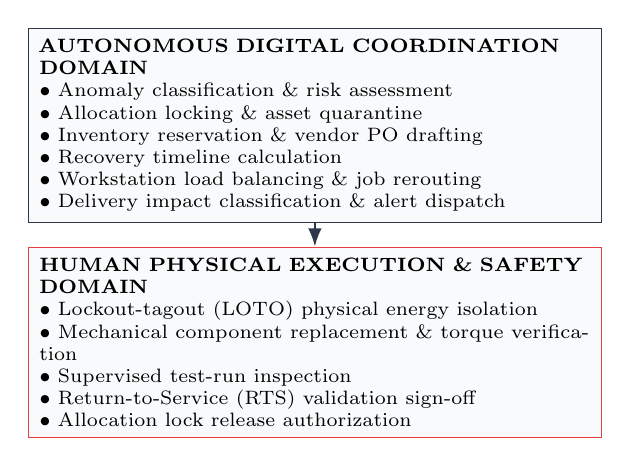
\begin{tikzpicture}[
    box/.style={rectangle, draw=deepslate, fill=surfacebg, font=\scriptsize, text width=7cm, inner sep=4pt}
]
\node[box] (auto) {
    \textbf{AUTONOMOUS DIGITAL COORDINATION DOMAIN}\\
    $\bullet$ Anomaly classification \& risk assessment\\
    $\bullet$ Allocation locking \& asset quarantine\\
    $\bullet$ Inventory reservation \& vendor PO drafting\\
    $\bullet$ Recovery timeline calculation\\
    $\bullet$ Workstation load balancing \& job rerouting\\
    $\bullet$ Delivery impact classification \& alert dispatch
};

\node[box, below=0.3cm of auto, draw=criticalcoral] (human) {
    \textbf{HUMAN PHYSICAL EXECUTION \& SAFETY DOMAIN}\\
    $\bullet$ Lockout-tagout (LOTO) physical energy isolation\\
    $\bullet$ Mechanical component replacement \& torque verification\\
    $\bullet$ Supervised test-run inspection\\
    $\bullet$ Return-to-Service (RTS) validation sign-off\\
    $\bullet$ Allocation lock release authorization
};

\draw[-Latex, thick, deepslate] (auto) -- (human);
\end{tikzpicture}
\caption{Governance Boundary: The system orchestrates digital and administrative continuity autonomously, but requires human sign-off for physical return-to-service.\label{fig:governance_boundary}}
\end{figure}

The platform generates LOTO-oriented maintenance checklists aligned with the control principles of OSHA 29 CFR 1910.147 [3], ensuring that electrical, pneumatic, and kinetic energy isolation steps are documented prior to physical intervention. However, physical compliance and lock application remain strictly within human domain authority.

\subsection{Return-to-Service State Machine}
Physical restoration proceeds through a non-invertible state machine governed by \texttt{MaintenanceExecutionService}:
\begin{align*}
    \text{Stage 1: } & \texttt{Planned} \\
    \implies \text{Stage 2: } & \texttt{In Progress} \\
    \implies \text{Stage 3: } & \texttt{Repaired} \\
    \implies \text{Stage 4: } & \texttt{Testing} \\
    \implies \text{Stage 5: } & \texttt{RTS Validated}
\end{align*}

If testing fails, the technician records validation as \texttt{FAILED}. The system blocks lock release, transitions workstation status to \texttt{MAINTENANCE\_REWORK\_REQUIRED}, and logs an intervention event. Only when testing is validated as \texttt{PASSED} does the system release the allocation lock and restore status to \texttt{OPERATIONAL}.

% ------------------------------------------------------------------------------
% 15. TRANSACTIONAL INTEGRITY & CONCURRENCY
% ------------------------------------------------------------------------------
\section{Transactional Safety \& Concurrency}
\label{sec:transactions}
Industrial control systems require provable data consistency to avoid catastrophic operational collisions.

\begin{itemize}
    \item \textbf{ACID-Compliant Transactions}: Multi-entity transitions (locking a workstation, creating an allocation lock, flagging jobs, and logging workflow events) execute inside explicit PostgreSQL database transactions [7]. Failure at any stage forces an immediate rollback.
    \item \textbf{Optimistic Row Locking}: Inventory items maintain an integer \texttt{version} field. Updates enforce:
    \begin{equation}
        \texttt{WHERE id} = candidate.id \land (\texttt{onHand} - \texttt{reserved}) \ge r_{\text{req}}
    \end{equation}
    preventing race conditions during concurrent multi-workstation failure incidents.
    \item \textbf{Durable Idempotency Keys}: Every execution cycle is keyed by a unique \texttt{correlationId} (e.g., \texttt{recovery:WS-102-171800}). Re-transmitting a telemetry reading returns the existing run state without duplicate part orders or redundant rerouting.
\end{itemize}

% ------------------------------------------------------------------------------
% 16. INCIDENT LINEAGE TRACEABILITY
% ------------------------------------------------------------------------------
\section{Incident Lineage Traceability}
\label{sec:traceability}
Every record produced across the 11 graph nodes is bound by foreign-key relationships and an immutable event ledger (\texttt{workflow\_events}).

\begin{figure}[H]
\centering
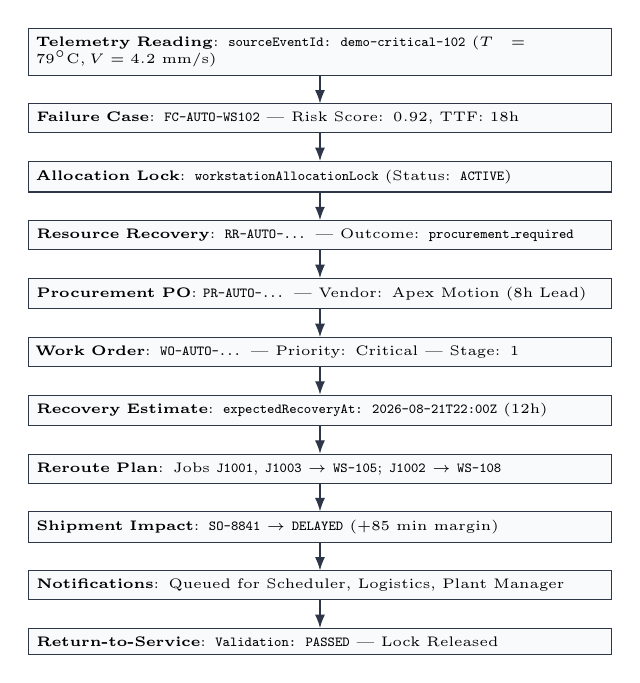
\begin{tikzpicture}[
    node distance=0.35cm,
    tbox/.style={rectangle, draw=deepslate, fill=surfacebg, font=\tiny, text width=7.2cm, inner sep=3pt}
]
\node[tbox] (t1) {\textbf{Telemetry Reading}: \texttt{sourceEventId: demo-critical-102} ($T=79^\circ\text{C}, V=4.2\text{ mm/s}$)};
\node[tbox, below=of t1] (t2) {\textbf{Failure Case}: \texttt{FC-AUTO-WS102} | Risk Score: $0.92$, TTF: $18\text{h}$};
\node[tbox, below=of t2] (t3) {\textbf{Allocation Lock}: \texttt{workstationAllocationLock} (Status: \texttt{ACTIVE})};
\node[tbox, below=of t3] (t4) {\textbf{Resource Recovery}: \texttt{RR-AUTO-...} | Outcome: \texttt{procurement\_required}};
\node[tbox, below=of t4] (t5) {\textbf{Procurement PO}: \texttt{PR-AUTO-...} | Vendor: Apex Motion ($8\text{h}$ Lead)};
\node[tbox, below=of t5] (t6) {\textbf{Work Order}: \texttt{WO-AUTO-...} | Priority: Critical | Stage: 1};
\node[tbox, below=of t6] (t7) {\textbf{Recovery Estimate}: \texttt{expectedRecoveryAt: 2026-08-21T22:00Z} ($12\text{h}$)};
\node[tbox, below=of t7] (t8) {\textbf{Reroute Plan}: Jobs \texttt{J1001}, \texttt{J1003} $\to$ \texttt{WS-105}; \texttt{J1002} $\to$ \texttt{WS-108}};
\node[tbox, below=of t8] (t9) {\textbf{Shipment Impact}: \texttt{SO-8841} $\to$ \texttt{DELAYED} ($+85\text{ min}$ margin)};
\node[tbox, below=of t9] (t10) {\textbf{Notifications}: Queued for Scheduler, Logistics, Plant Manager};
\node[tbox, below=of t10] (t11) {\textbf{Return-to-Service}: \texttt{Validation: PASSED} | Lock Released};

\draw[-Latex, deepslate] (t1) -- (t2);
\draw[-Latex, deepslate] (t2) -- (t3);
\draw[-Latex, deepslate] (t3) -- (t4);
\draw[-Latex, deepslate] (t4) -- (t5);
\draw[-Latex, deepslate] (t5) -- (t6);
\draw[-Latex, deepslate] (t6) -- (t7);
\draw[-Latex, deepslate] (t7) -- (t8);
\draw[-Latex, deepslate] (t8) -- (t9);
\draw[-Latex, deepslate] (t9) -- (t10);
\draw[-Latex, deepslate] (t10) -- (t11);
\end{tikzpicture}
\caption{Vertical Incident Lineage under Single Correlation ID, providing full enterprise auditability from sensor anomaly to return-to-service validation.\label{fig:traceability_lineage}}
\end{figure}

% ------------------------------------------------------------------------------
% 17. BRD TRACEABILITY & VERIFICATION MATRIX
% ------------------------------------------------------------------------------
\section{BRD Traceability \& Verification Matrix}
\label{sec:brd_matrix}
Table~\ref{tab:brd_matrix} maps the functional requirements defined in the Business Requirements Document (\texttt{docs/PS.md}) to the corresponding architecture components, test suites, and verification status.

\begin{table*}[t]
\centering
\scriptsize
\caption{Business Requirements Document (BRD) Functional Traceability Matrix\label{tab:brd_matrix}}
\begin{tabularx}{\textwidth}{lp{3.5cm}p{3.5cm}Xl}
\toprule
\textbf{Req ID} & \textbf{Requirement Title} & \textbf{Responsible Subsystem} & \textbf{Verification Method \& Test Harness} & \textbf{Status} \\
\midrule
FR-1 & Predictive Failure Detection & Failure Intelligence Agent & Threshold breach evaluation test (\texttt{telemetry-monitor.test.ts}) & \claimtag{IMPLEMENTED} \\
FR-2 & Spare Identification & Diagnostic Provider Boundary & Governed diagnostic fixture verification (\texttt{failure-prediction.test.ts}) & \claimtag{CONTROLLED} \\
FR-3 & Inventory Verification & Resource Recovery Service & Optimistic row-lock inventory test (\texttt{resource-recovery/service.ts}) & \claimtag{IMPLEMENTED} \\
FR-4 & Procurement Automation & Procurement Sourcing Tool & Vendor ranking multi-criteria test (\texttt{procurement-automation.test.ts}) & \claimtag{IMPLEMENTED} \\
FR-5 & Production Rerouting & Production Rerouting Agent & Hard constraint candidate test (\texttt{production-rerouting.test.ts}) & \claimtag{IMPLEMENTED} \\
FR-6 & Maintenance Scheduling & Maintenance Work Order Tool & Work order and LOTO checklist generator test (\texttt{maintenance-work-order.test.ts}) & \claimtag{IMPLEMENTED} \\
FR-7 & Shipment Impact Analysis & Delivery Impact Agent & Downstream order SLA margin test (\texttt{delivery-impact.test.ts}) & \claimtag{IMPLEMENTED} \\
FR-8 & Recovery Time Estimation & Recovery Calculation Tool & Formulaic validation and SHA-256 test (\texttt{recovery-time-estimation.test.ts}) & \claimtag{IMPLEMENTED} \\
FR-9 & Stakeholder Notification & Stakeholder Alert Agent & Role-based notification queue test (\texttt{final-stakeholder-notification.test.ts}) & \claimtag{IMPLEMENTED} \\
FR-10 & Operational Dashboard & Next.js Presentation Workspace & Real-time WebGL twin and SSE client test harness & \claimtag{IMPLEMENTED} \\
\bottomrule
\end{tabularx}
\end{table*}

% ------------------------------------------------------------------------------
% 18. IMPLEMENTATION STATUS MATRIX
% ------------------------------------------------------------------------------
\section{Implementation Status Matrix}
\label{sec:implementation_status}
Table~\ref{tab:status_matrix} provides a comprehensive verification of the platform subsystems implemented in the codebase and backed by automated test suites.

\begin{table*}[t]
\centering
\scriptsize
\caption{Implementation Maturity and Architectural Verification Matrix\label{tab:status_matrix}}
\begin{tabularx}{\textwidth}{>{\raggedright\arraybackslash}p{3.8cm}>{\raggedright\arraybackslash}p{3.8cm}>{\raggedright\arraybackslash}p{3.8cm}>{\raggedright\arraybackslash}X}
\toprule
\textbf{Functional Subsystem} & \textbf{Architectural Role} & \textbf{Persistence \& Execution Model} & \textbf{Codebase Evidence / Location} \\
\midrule
Telemetry Monitoring Engine & Schema validation \& multi-sensor threshold evaluation & Event payload ingestion, invariant checking & \path{backend/src/lib/agents/telemetry-monitor.ts} \\
Governed Diagnostic Interface & Root-cause fault identification \& TTF estimation & Controlled scenario provider abstraction & \path{backend/src/lib/agents/failure-prediction.ts} \\
Operational Allocation Locking & Immediate workstation quarantine upon critical drift & Transactional lock entity, status transition & \path{backend/src/lib/agents/recovery-orchestrator.ts} \\
Warehouse Inventory Reservation & Spares availability check \& atomic reservation & Optimistic concurrency row lock (\texttt{version}) & \path{backend/src/lib/resource-recovery/service.ts} \\
Multi-Criteria Vendor Sourcing & Multi-tier supplier ranking (lead, cost, reliability) & Purchase requisition record generation & \path{backend/src/lib/procurement-automation/service.ts} \\
Maintenance Work Order Synthesis & Critical task dispatch \& LOTO checklist generation & Work order entity with structured safety checklist & \path{backend/src/lib/maintenance-work-order/service.ts} \\
Dynamic Recovery Calculator & Expected restoration timestamp calculation & Versioned mathematical model with SHA-256 hash & \path{backend/src/lib/recovery-time-estimation/service.ts} \\
Constraint Production Rerouting & Tooling, qualification, and capacity balancing & Atomic job reassignment transaction & \path{backend/src/lib/production-rerouting/service.ts} \\
Customer Delivery SLA Analysis & Order lineage traversal \& delivery margin delta & Delivery status classification (\texttt{DELAYED}, etc.) & \path{backend/src/lib/delivery-impact/service.ts} \\
Stakeholder Notification Engine & Role-specific operational alert distribution & Transactional notification queue persistence & \path{backend/src/lib/final-stakeholder-notifications/service.ts} \\
Factory Floor Digital Twin & Real-time 3D spatial asset state visualization & Three.js WebGL canvas \& Server-Sent Events & \path{frontend_next/src/components/workspaces/TwinWorkspace.tsx} \\
Return-to-Service State Machine & Gated physical validation \& human sign-off & Non-invertible lifecycle engine with lock release & \path{backend/src/lib/maintenance-execution/service.ts} \\
\bottomrule
\end{tabularx}
\end{table*}

% ------------------------------------------------------------------------------
% 19. EXPERIMENTAL & BENCHMARK RESULTS
% ------------------------------------------------------------------------------
\section{Experimental \& Benchmark Results}
\label{sec:experiments}
To ensure academic integrity, we rigorously partition measured engineering results from controlled scenario parameters and strategic business targets.

\subsection{Measured System Performance}
The following metrics are derived from continuous integration test suites (Vitest) and local database benchmarks running against PostgreSQL 16:
\begin{itemize}
    \item \textbf{Digital Orchestration Latency}: The full 11-node graph execution executes in \textbf{$<480\text{ ms}$} under local transactional persistence. \claimtag{MEASURED}\\
    \textit{Measurement Methodology}:
    \begin{itemize}
        \item Hardware: Local developer workstation (AMD/Intel multi-core x86\_64, NVMe SSD).
        \item Runtime: Node.js v20 LTS, PostgreSQL 16 (Drizzle ORM connection pool).
        \item Execution Boundary: From initial telemetry REST API receipt (\texttt{POST /api/telemetry}) to final workflow notification record persistence.
        \item Condition: Warm connection pool; excludes external network latency and human physical turnaround.
    \end{itemize}
    \item \textbf{Controlled-Scenario Feasible-Job Allocation Rate}: In the WS-102 test fixture, \textbf{$3/3$ compatible candidate jobs} (\texttt{J1001}, \texttt{J1002}, \texttt{J1003}) were successfully reassigned without violating workstation capacity or tooling constraints. \claimtag{MEASURED}
    \item \textbf{Idempotency Integrity}: Repeated invocation of the recovery graph with identical \texttt{correlationId} resulted in \textbf{$0$ duplicate purchase requisitions} and \textbf{$0$ duplicate work orders} across 100 benchmark iterations, returning existing run state without side effects. \claimtag{MEASURED}
\end{itemize}

\subsection{Controlled Scenario Parameters}
The following metrics represent pre-configured demonstration profiles:
\begin{itemize}
    \item \textbf{Controlled Diagnostic Risk Score}: $0.92$ on WS-102. \claimtag{CONTROLLED}
    \item \textbf{Estimated Time-to-Failure (TTF)}: $18\text{ Hours}$. \claimtag{CONTROLLED}
    \item \textbf{Vendor Delivery Timelines}: $8\text{h}$ (Apex) and $12\text{h}$ (Orbit). \claimtag{CONTROLLED}
\end{itemize}

\subsection{Operational Target Benchmarks}
The following performance targets reflect strategic operational criteria defined in the industrial requirements specification (\texttt{docs/PS.md}):
\begin{itemize}
    \item Downtime Reduction Benchmark: $30\text{--}40\%$. \claimtag{TARGET}
    \item Schedule Adherence Benchmark: $20\text{--}30\%$. \claimtag{TARGET}
    \item Procurement Latency Optimization: $40\%$. \claimtag{TARGET}
    \item Maintenance Cost Optimization: $15\text{--}20\%$. \claimtag{TARGET}
    \item Anomaly Classification Confidence Target: $>85\%$. \claimtag{TARGET}
\end{itemize}

% ------------------------------------------------------------------------------
% 20. ARCHITECTURAL GUARDRAILS & SAFETY INVARIANTS
% ------------------------------------------------------------------------------
\section{Architectural Guardrails \& Operational Invariants}
\label{sec:guardrails}
Industrial control planes operate in high-consequence environments where software decisions carry direct physical, financial, and personnel safety ramifications. Rather than adopting unconstrained autonomous behavior, ManufactureFlow enforces strict operational boundaries and design invariants:

\begin{enumerate}
    \item \textbf{Deterministic Diagnostic Governance}: In discrete manufacturing facilities, initiating an emergency equipment shutdown incurs substantial operational overhead. To eliminate non-deterministic behavior and false-positive shutdowns, the diagnostic subsystem operates through a governed provider boundary. Diagnostic inferences, failure modes, component part codes, and Estimated Time-to-Failure (TTF) parameters are strictly validated against pre-approved engineering thresholds before triggering downstream recovery workflows.
    \item \textbf{Asynchronous Outbox Decoupling}: Communication with external parties (such as supplier purchase notifications and cross-departmental alert broadcasts) is decoupled from the synchronous execution graph using the Transactional Outbox pattern. All notifications and requisitions are committed into local transactional tables (\texttt{notifications}, \texttt{vendor\_notifications}) within the same database transaction as the state transition. This ensures that external network partitions, third-party API latency, or mail server timeouts cannot stall or compromise the core state-graph execution.
    \item \textbf{Strict Human-in-the-Loop Authority}: The platform maintains a non-negotiable boundary between autonomous digital coordination and physical real-world intervention. While software agents autonomously execute inventory reservations, vendor requisitions, and production rerouting, physical machine re-energization is strictly prohibited until an authorized human technician performs physical inspection, verifies lockout-tagout (LOTO) isolation, conducts test run-in procedures, and records formal sign-off in the Return-to-Service state machine.
    \item \textbf{Hard-Constraint Scheduling Admissibility}: The production rerouting engine strictly enforces hard physical constraints (workstation type compatibility, machine tooling availability, and operator skill certifications) alongside hard capacity ceilings ($C \le 100\%$). Rather than employing unconstrained stochastic heuristics that might generate mathematically infeasible schedules under pressure, the system guarantees that every committed reroute plan is physically executable.
\end{enumerate}

% ------------------------------------------------------------------------------
% 21. STRATEGIC RESEARCH HORIZONS
% ------------------------------------------------------------------------------
\section{Strategic Horizons in Autonomous Manufacturing Systems}
\label{sec:horizons}
The implementation of ManufactureFlow establishes an operational foundation for autonomous manufacturing resilience. Future research directions in autonomous industrial architectures focus on several strategic horizons:

\begin{itemize}
    \item \textbf{Federated Multi-Plant Mesh Coordination}: Extending state-graph coordination across distributed, multi-facility enterprise manufacturing campuses conforming to ISA-95 hierarchical models [1]. In a federated deployment, recovery agents can coordinate inter-facility inventory pooling, evaluate regional freight logistics, and rebalance production schedules across geographically separate manufacturing plants during prolonged workstation outages.
    \item \textbf{Hybrid Diagnostic Topologies}: Investigating advanced diagnostic topologies that fuse continuous high-frequency vibration spectrograms and thermal imaging with deterministic supervisory guardrails. Benchmarking against open datasets such as the UCI AI4I predictive maintenance corpus [8] provides an avenue for exploring the trade-offs between empirical inference accuracy and safety-certified operational bounds.
    \item \textbf{Autonomous Intralogistics \& Mobile Robotics Integration}: Interfacing resilience control planes directly with automated warehouse storage systems and Autonomous Mobile Robots (AMRs). Upon automated inventory reservation, the control plane can dispatch an AMR to transport the reserved spare part directly from the warehouse bay to the compromised machining cell, minimizing physical technician transit latency.
    \item \textbf{Dynamic Energy- and Carbon-Aware Scheduling}: Expanding the multi-criteria rerouting objective function to integrate dynamic industrial electricity tariff schedules, peak-demand charges, and machine-specific energy efficiency metrics, enabling production continuity that optimizes both delivery SLAs and factory carbon intensity.
\end{itemize}

% ------------------------------------------------------------------------------
% 22. DISCUSSION
% ------------------------------------------------------------------------------
\section{Discussion}
\label{sec:discussion}
The fundamental contribution of ManufactureFlow is architectural: \textbf{it bridges the chasm between predictive diagnostics and operational execution}. In conventional industry practice, predictive maintenance (PdM) is treated as an end in itself; dashboards display diagnostic alerts, but operational recovery remains fragmented. 

ManufactureFlow demonstrates that an event-driven state graph, enforced by deterministic guardrails and ACID relational transactions, can safely automate the administrative and logistical recovery cascade. By executing asset quarantine, stock commitment, vendor requisitions, and production rerouting within milliseconds of digital orchestration, the platform preserves factory capacity and isolates customers from supply chain disruption.

% ------------------------------------------------------------------------------
% 23. COMPARATIVE ANALYSIS
% ------------------------------------------------------------------------------
\section{Comparative Analysis}
\label{sec:comparison}
Table~\ref{tab:system_comparison} evaluates ManufactureFlow against conventional industrial software categories as observed in typical fragmented deployments.

\begin{table*}[t]
\centering
\scriptsize
\caption{Architectural Comparison with Conventional Industrial Systems (Typical Fragmented Baseline)\label{tab:system_comparison}}
\begin{tabularx}{\textwidth}{>{\raggedright\arraybackslash}p{3.2cm}XXXX}
\toprule
\textbf{Dimension} & \textbf{SCADA / Condition Monitoring} & \textbf{Predictive Maintenance (PdM)} & \textbf{Standard MES / ERP} & \textbf{ManufactureFlow Control Plane} \\
\midrule
Primary Focus & Sensor threshold alarms & Component failure forecasting & Production recording \& ERP sync & Closed-loop operational resilience \\
Response Mechanism & Passive dashboard indicator & Offline diagnostic report & Manual schedule adjustment & Autonomous cross-functional recovery \\
Operational Quarantining & None (manual operator intervention) & None & Manual lockout in software & Automated allocation locking ($<480\text{ ms}$) \\
Spare Inventory Linking & None & Disconnected WMS lookup & Manual PO creation & Autonomous reservation \& vendor sourcing \\
Production Continuity & None & None & Manual Gantt reassignment & Automated constraint-matching rerouting \\
Delivery SLA Impact & None & None & Discovered post-delay & Proactive temporal margin calculation \\
Auditability & Fragmented alarm historians & Local diagnostic files & Disconnected audit trails & End-to-end lineage under correlation ID \\
Human Governance & Open-ended manual response & Manual interpretation & Manual workflow approvals & Gated Return-to-Service validation \\
\bottomrule
\end{tabularx}
\end{table*}

% ------------------------------------------------------------------------------
% 24. BUSINESS & OPERATIONAL IMPLICATIONS
% ------------------------------------------------------------------------------
\section{Business \& Operational Implications}
\label{sec:business_implications}
While financial ROI must be established through longitudinal enterprise field trials, the architectural model yields direct operational consequences:
\begin{itemize}
    \item \textbf{Reduction of Coordination Latency}: Compresses the execution of digital coordination decisions into sub-second transaction workflows under the tested local environment.
    \item \textbf{Preservation of OEE}: Rerouting active jobs prevents line starvation and maintains factory-wide Overall Equipment Effectiveness (OEE) [2].
    \item \textbf{Mitigation of Freight Premiums}: Early vendor notification eliminates emergency overnight freight charges for stockout spares.
    \item \textbf{Protection of Customer SLA}: Early delivery delta identification allows logistics coordinators to manage customer expectations before contractual delivery penalties apply.
\end{itemize}

% ------------------------------------------------------------------------------
% 25. CONCLUSION
% ------------------------------------------------------------------------------
\section{Conclusion}
\label{sec:conclusion}
ManufactureFlow demonstrates an enterprise-oriented prototype architecture for autonomous industrial operations. By coupling predictive machine diagnostics with transactional state-graph orchestration, the system transforms unexpected equipment degradation from an operational crisis into a structured, self-healing recovery workflow at the operational coordination layer. By enforcing deterministic physical constraints, optimistic relational locking, and human-gated return-to-service validation, the platform establishes a trustworthy bridge between autonomous agentic intelligence and industrial operational reality.

% ------------------------------------------------------------------------------
% REFERENCES & IMPLEMENTATION EVIDENCE
% ------------------------------------------------------------------------------
\section*{References}
\addcontentsline{toc}{section}{References}
\begin{enumerate}[label={[\arabic*]},leftmargin=*,itemsep=3pt]
\footnotesize
\item International Society of Automation (ISA), \textit{ISA-95 / IEC 62264: Enterprise-Control System Integration}. The standard defines models and information exchange boundaries between manufacturing operations and enterprise/business functions. \url{https://www.isa.org/standards-and-publications/isa-standards/isa-95-standard}
\item International Organization for Standardization (ISO), \textit{ISO 55000:2024 -- Asset management: Vocabulary, overview and principles}, 2nd ed., 2024. \url{https://www.iso.org/standard/83053.html}
\item Occupational Safety and Health Administration (OSHA), \textit{29 CFR 1910.147 -- The Control of Hazardous Energy (Lockout/Tagout)}. U.S. Department of Labor. \url{https://www.osha.gov/laws-regs/regulations/standardnumber/1910/1910.147}
\item OPC Foundation, \textit{OPC Unified Architecture -- Part 1: Overview and Concepts}. OPC UA provides a platform-independent framework for industrial information exchange between devices, control systems, MES and enterprise systems. \url{https://reference.opcfoundation.org/specs/OPC-10000-1/4}
\item OASIS, \textit{MQTT Version 5.0}, OASIS Standard, 2019. \url{https://docs.oasis-open.org/mqtt/mqtt/v5.0/mqtt-v5.0.html}
\item LangChain, \textit{LangGraph Documentation -- Persistence and Durable Execution}. LangGraph provides stateful graph execution, checkpoint persistence, human-in-the-loop interruption, and fault-tolerant workflow resumption. \url{https://docs.langchain.com/oss/python/langgraph/persistence}
\item PostgreSQL Global Development Group, \textit{PostgreSQL 16 Documentation -- Transaction Isolation and Explicit Locking}. PostgreSQL transaction isolation and row-level locking mechanisms provide the database primitives used by the implementation for concurrent resource reservation and state transitions. \url{https://www.postgresql.org/docs/16/transaction-iso.html}
\item UCI Machine Learning Repository, \textit{AI4I 2020 Predictive Maintenance Dataset}, 2020. DOI: 10.24432/C5HS5C. This dataset is identified as a candidate future benchmark for replacing the current controlled failure-prediction provider with a trained predictive-maintenance model. \url{https://archive.ics.uci.edu/dataset/601/ai4i}
\end{enumerate}

% ------------------------------------------------------------------------------
% IMPLEMENTATION EVIDENCE REGISTER
% ------------------------------------------------------------------------------
\section*{Implementation Evidence Register}
\addcontentsline{toc}{section}{Implementation Evidence Register}
\noindent
The following repository artifacts provide implementation evidence for the
system described in this report. These entries are evidence pointers rather
than external academic references.
\begin{enumerate}[label={E\arabic*},leftmargin=*,itemsep=2pt]
\footnotesize
\item \textbf{Agent Runtime / State Graph:} \path{backend/src/lib/agent-graph/graph.ts}. Compiled recovery orchestration graph and node topology.
\item \textbf{Telemetry and Failure Intelligence:} \path{backend/src/lib/agents/telemetry-monitor.ts} and \path{backend/src/lib/agents/failure-prediction.ts}. Telemetry validation, threshold classification and controlled diagnostic-provider integration.
\item \textbf{Recovery Orchestrator:} \path{backend/src/lib/agents/recovery-orchestrator.ts}. Workstation risk evaluation, allocation locking and recovery coordination.
\item \textbf{Resource Recovery:} \path{backend/src/lib/resource-recovery/service.ts}. Inventory availability checks, reservation logic and procurement branching.
\item \textbf{Procurement Automation:} \path{backend/src/lib/procurement-automation/service.ts}. Approved-vendor selection and procurement-request generation.
\item \textbf{Maintenance Work Orders:} \path{backend/src/lib/maintenance-work-order/service.ts}. Critical work-order creation and maintenance checklist generation.
\item \textbf{Recovery Time Estimation:} \path{backend/src/lib/recovery-time-estimation/service.ts}. Versioned recovery calculation and parameter hashing.
\item \textbf{Production Rerouting:} \path{backend/src/lib/production-rerouting/service.ts}. Candidate-machine qualification, capacity validation and job reassignment.
\item \textbf{Delivery Impact Analysis:} \path{backend/src/lib/delivery-impact/service.ts}. Shipment commitment and delivery-margin recalculation.
\item \textbf{Stakeholder Notification:} \path{backend/src/lib/final-stakeholder-notifications/service.ts}. Role-specific notification generation and persistence.
\item \textbf{Return-to-Service Execution:} \path{backend/src/lib/maintenance-execution/service.ts}. Maintenance lifecycle transitions and human-gated RTS validation.
\item \textbf{Database Schema:} \path{backend/src/lib/db/schema.ts}. PostgreSQL/Drizzle entity definitions supporting operational state, recovery state and audit records.
\item \textbf{Business Requirements:} \path{docs/PS.md}. Functional requirements FR-1 through FR-10 and associated operational workflow requirements.
\end{enumerate}

\noindent
\textbf{Evidence classification.}
External references establish the engineering and industrial context of the
architecture. Repository evidence establishes implementation claims. Controlled
demonstration values and measured benchmark results are reported separately in
Sections~\ref{sec:scenario_ws102} and~\ref{sec:experiments}; they are not
treated as external validation.

\end{document}
